\begin{figure}[t]
	\centering
	\begin{minipage}{0.48\linewidth}
		\centering
   		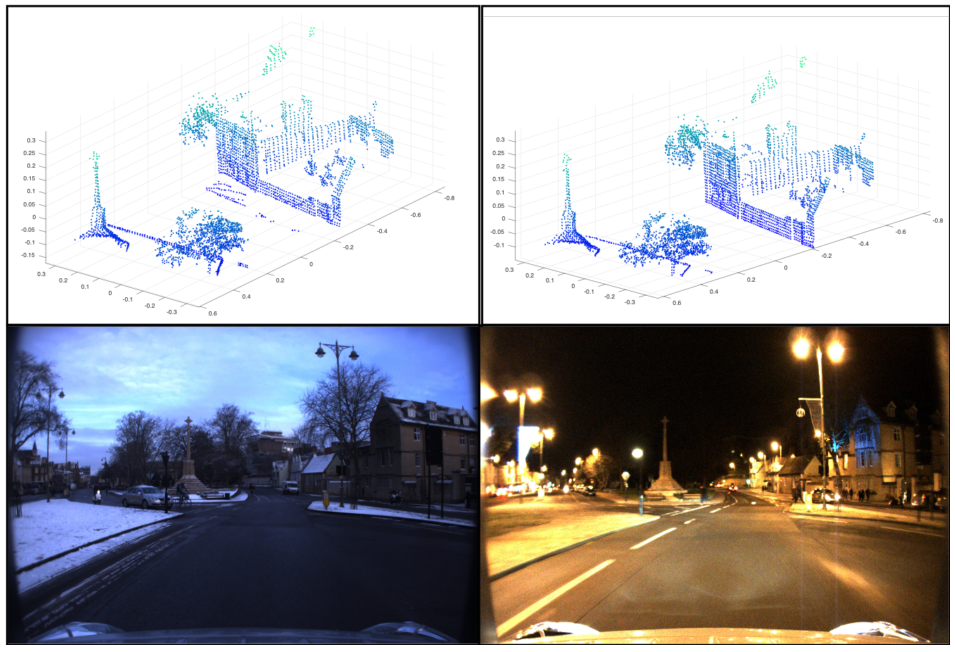
\includegraphics[width=\linewidth]{data_hetero/pointnetvlad.png}
	   		
   		\noindent\rule{\linewidth}{0.4pt}
   		   		
   		\subfigure[][Geometric information]{\label{fig:3d_info}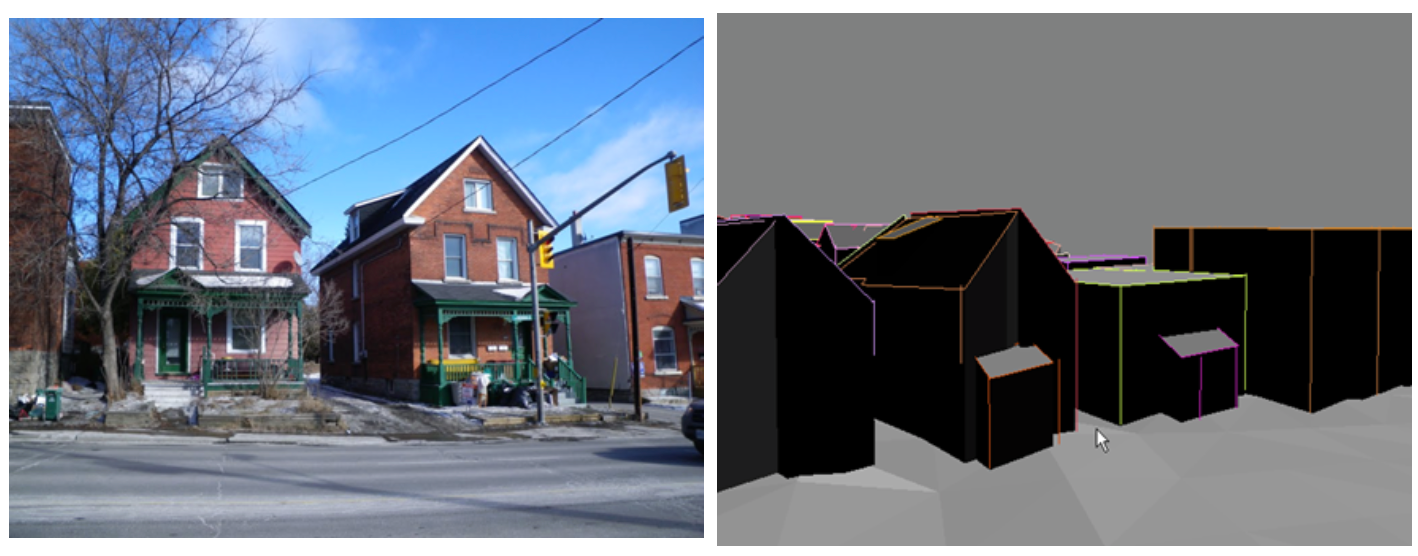
\includegraphics[width=\linewidth]{data_hetero/image_to_DEM.png}}
	\end{minipage}
	\begin{minipage}{0.48\linewidth}
		\centering
   		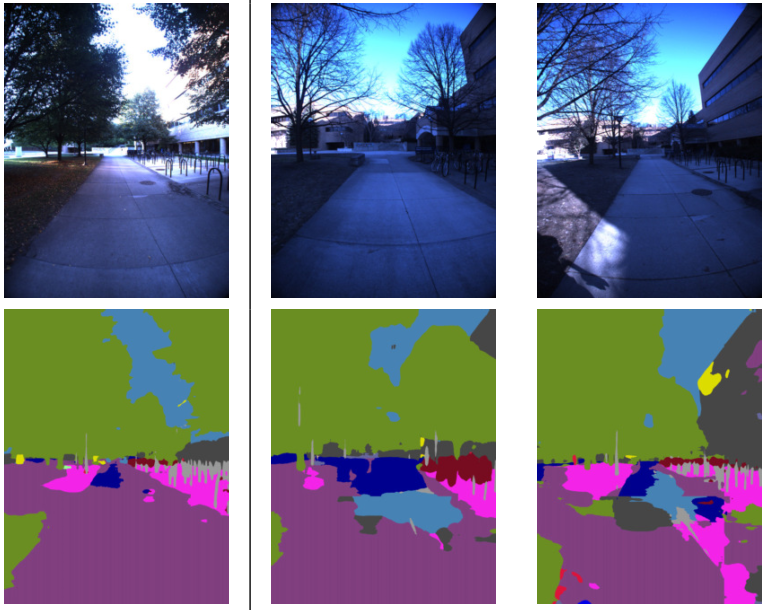
\includegraphics[width=0.95\linewidth]{data_hetero/semantic_vbl.png}
   		
		\noindent\rule{\linewidth}{0.4pt}		
		
   		\subfigure[][Semantic information]{\label{fig:seg_ifo}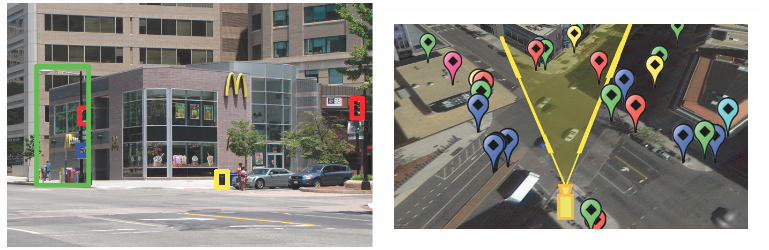
\includegraphics[width=\linewidth]{data_hetero/semantic.png}}
	\end{minipage}
	\caption[Illustration of the data heterogeneity in \ac{vbl}]{\textbf{Illustration of the data heterogeneity in \ac{vbl}:} \ref{fig:3d_info}~From top to bottom: PointNetVLAD~\citep{Uy2018} used to match point cloud for \acs{vbl} and localization system built upon a DEM~\citep{Matei2013}. \ref{fig:seg_ifo}~From top to bottom: data segmentation to help queries (right) to database (left) visual association~\citep{Schonberger2017a} and localization system with semantic information gathered from OpenStreetMap annotation~\citep{Ardeshir2014}. \label{fig:data_div}}
\end{figure}